% Created by tikzDevice version 0.8 on 2015-01-07 01:15:50
% !TEX encoding = UTF-8 Unicode
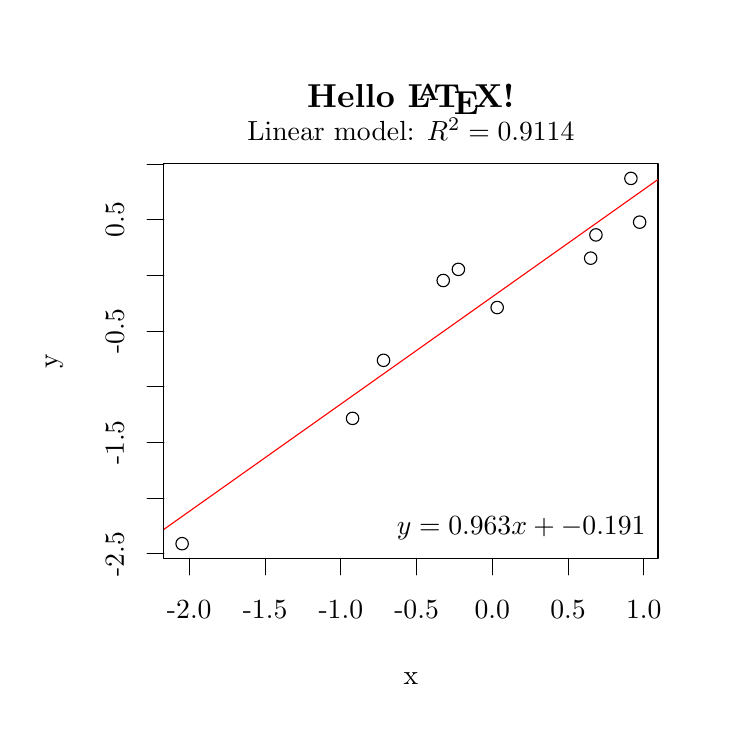
\begin{tikzpicture}[x=1pt,y=1pt]
\definecolor{fillColor}{RGB}{255,255,255}
\path[use as bounding box,fill=fillColor,fill opacity=0.00] (0,0) rectangle (252.94,252.94);
\begin{scope}
\path[clip] ( 49.20, 61.20) rectangle (227.75,203.75);
\definecolor{drawColor}{RGB}{0,0,0}

\path[draw=drawColor,line width= 0.4pt,line join=round,line cap=round] (150.16,161.58) circle (  2.25);

\path[draw=drawColor,line width= 0.4pt,line join=round,line cap=round] (217.98,198.47) circle (  2.25);

\path[draw=drawColor,line width= 0.4pt,line join=round,line cap=round] (117.40,111.76) circle (  2.25);

\path[draw=drawColor,line width= 0.4pt,line join=round,line cap=round] (205.34,178.05) circle (  2.25);

\path[draw=drawColor,line width= 0.4pt,line join=round,line cap=round] (221.13,182.66) circle (  2.25);

\path[draw=drawColor,line width= 0.4pt,line join=round,line cap=round] (155.64,165.60) circle (  2.25);

\path[draw=drawColor,line width= 0.4pt,line join=round,line cap=round] (128.58,132.74) circle (  2.25);

\path[draw=drawColor,line width= 0.4pt,line join=round,line cap=round] ( 55.81, 66.48) circle (  2.25);

\path[draw=drawColor,line width= 0.4pt,line join=round,line cap=round] (169.65,151.81) circle (  2.25);

\path[draw=drawColor,line width= 0.4pt,line join=round,line cap=round] (203.44,169.65) circle (  2.25);
\end{scope}
\begin{scope}
\path[clip] (  0.00,  0.00) rectangle (252.94,252.94);
\definecolor{drawColor}{RGB}{0,0,0}

\path[draw=drawColor,line width= 0.4pt,line join=round,line cap=round] ( 58.40, 61.20) -- (222.65, 61.20);

\path[draw=drawColor,line width= 0.4pt,line join=round,line cap=round] ( 58.40, 61.20) -- ( 58.40, 55.20);

\path[draw=drawColor,line width= 0.4pt,line join=round,line cap=round] ( 85.78, 61.20) -- ( 85.78, 55.20);

\path[draw=drawColor,line width= 0.4pt,line join=round,line cap=round] (113.15, 61.20) -- (113.15, 55.20);

\path[draw=drawColor,line width= 0.4pt,line join=round,line cap=round] (140.52, 61.20) -- (140.52, 55.20);

\path[draw=drawColor,line width= 0.4pt,line join=round,line cap=round] (167.90, 61.20) -- (167.90, 55.20);

\path[draw=drawColor,line width= 0.4pt,line join=round,line cap=round] (195.27, 61.20) -- (195.27, 55.20);

\path[draw=drawColor,line width= 0.4pt,line join=round,line cap=round] (222.65, 61.20) -- (222.65, 55.20);

\node[text=drawColor,anchor=base,inner sep=0pt, outer sep=0pt, scale=  1.00] at ( 58.40, 39.60) {-2.0};

\node[text=drawColor,anchor=base,inner sep=0pt, outer sep=0pt, scale=  1.00] at ( 85.78, 39.60) {-1.5};

\node[text=drawColor,anchor=base,inner sep=0pt, outer sep=0pt, scale=  1.00] at (113.15, 39.60) {-1.0};

\node[text=drawColor,anchor=base,inner sep=0pt, outer sep=0pt, scale=  1.00] at (140.52, 39.60) {-0.5};

\node[text=drawColor,anchor=base,inner sep=0pt, outer sep=0pt, scale=  1.00] at (167.90, 39.60) {0.0};

\node[text=drawColor,anchor=base,inner sep=0pt, outer sep=0pt, scale=  1.00] at (195.27, 39.60) {0.5};

\node[text=drawColor,anchor=base,inner sep=0pt, outer sep=0pt, scale=  1.00] at (222.65, 39.60) {1.0};

\path[draw=drawColor,line width= 0.4pt,line join=round,line cap=round] ( 49.20, 62.77) -- ( 49.20,203.65);

\path[draw=drawColor,line width= 0.4pt,line join=round,line cap=round] ( 49.20, 62.77) -- ( 43.20, 62.77);

\path[draw=drawColor,line width= 0.4pt,line join=round,line cap=round] ( 49.20, 82.90) -- ( 43.20, 82.90);

\path[draw=drawColor,line width= 0.4pt,line join=round,line cap=round] ( 49.20,103.02) -- ( 43.20,103.02);

\path[draw=drawColor,line width= 0.4pt,line join=round,line cap=round] ( 49.20,123.15) -- ( 43.20,123.15);

\path[draw=drawColor,line width= 0.4pt,line join=round,line cap=round] ( 49.20,143.27) -- ( 43.20,143.27);

\path[draw=drawColor,line width= 0.4pt,line join=round,line cap=round] ( 49.20,163.40) -- ( 43.20,163.40);

\path[draw=drawColor,line width= 0.4pt,line join=round,line cap=round] ( 49.20,183.52) -- ( 43.20,183.52);

\path[draw=drawColor,line width= 0.4pt,line join=round,line cap=round] ( 49.20,203.65) -- ( 43.20,203.65);

\node[text=drawColor,rotate= 90.00,anchor=base,inner sep=0pt, outer sep=0pt, scale=  1.00] at ( 34.80, 62.77) {-2.5};

\node[text=drawColor,rotate= 90.00,anchor=base,inner sep=0pt, outer sep=0pt, scale=  1.00] at ( 34.80,103.02) {-1.5};

\node[text=drawColor,rotate= 90.00,anchor=base,inner sep=0pt, outer sep=0pt, scale=  1.00] at ( 34.80,143.27) {-0.5};

\node[text=drawColor,rotate= 90.00,anchor=base,inner sep=0pt, outer sep=0pt, scale=  1.00] at ( 34.80,183.52) {0.5};

\path[draw=drawColor,line width= 0.4pt,line join=round,line cap=round] ( 49.20, 61.20) --
	(227.75, 61.20) --
	(227.75,203.75) --
	( 49.20,203.75) --
	( 49.20, 61.20);
\end{scope}
\begin{scope}
\path[clip] (  0.00,  0.00) rectangle (252.94,252.94);
\definecolor{drawColor}{RGB}{0,0,0}

\node[text=drawColor,anchor=base,inner sep=0pt, outer sep=0pt, scale=  1.20] at (138.47,224.20) {\bfseries Hello \LaTeX!};

\node[text=drawColor,anchor=base,inner sep=0pt, outer sep=0pt, scale=  1.00] at (138.47, 15.60) {x};

\node[text=drawColor,rotate= 90.00,anchor=base,inner sep=0pt, outer sep=0pt, scale=  1.00] at ( 10.80,132.47) {y};
\end{scope}
\begin{scope}
\path[clip] ( 49.20, 61.20) rectangle (227.75,203.75);
\definecolor{drawColor}{RGB}{255,0,0}

\path[draw=drawColor,line width= 0.4pt,line join=round,line cap=round] ( 49.20, 71.64) -- (227.75,198.07);
\end{scope}
\begin{scope}
\path[clip] (  0.00,  0.00) rectangle (252.94,252.94);
\definecolor{drawColor}{RGB}{0,0,0}

\node[text=drawColor,anchor=base,inner sep=0pt, outer sep=0pt, scale=  1.00] at (138.47,212.14) {Linear model: $R^{2}= 0.9114 $};
\end{scope}
\begin{scope}
\path[clip] ( 49.20, 61.20) rectangle (227.75,203.75);
\definecolor{drawColor}{RGB}{0,0,0}

\node[text=drawColor,anchor=base west,inner sep=0pt, outer sep=0pt, scale=  1.00] at (133.38, 69.76) {$y = 0.963x +-0.191$};
\end{scope}
\end{tikzpicture}
